
\documentclass[11pt]{article}

%Menge: \mathbb{R}

\usepackage[ngerman]{babel}
\usepackage{amsmath} %align, für = untereinander einfach &=
\usepackage{amssymb}
\usepackage{amsthm}
\usepackage{listings}
\usepackage{pdfpages}
\usepackage[utf8]{inputenc}
\usepackage{graphicx}
\usepackage{esvect}
\graphicspath{ {./images/} }
\usepackage{tcolorbox}
\usepackage{tikz}         % For arrow and dots in \xvec
\usepackage[left=2.30cm, right=2.30cm, top=1.70cm, bottom=2.00cm]{geometry}

% --- Macro \xvec
\makeatletter
\newlength\xvec@height%
\newlength\xvec@depth%
\newlength\xvec@width%
\newcommand{\xvec}[2][]{%
	\ifmmode%
	\settoheight{\xvec@height}{$#2$}%
	\settodepth{\xvec@depth}{$#2$}%
	\settowidth{\xvec@width}{$#2$}%
	\else%
	\settoheight{\xvec@height}{#2}%
	\settodepth{\xvec@depth}{#2}%
	\settowidth{\xvec@width}{#2}%
	\fi%
	\def\xvec@arg{#1}%
	\def\xvec@dd{:}%
	\def\xvec@d{.}%
	\raisebox{.2ex}{\raisebox{\xvec@height}{\rlap{%
				\kern.05em%  (Because left edge of drawing is at .05em)
				\begin{tikzpicture}[scale=1]
				\pgfsetroundcap
				\draw (.05em,0)--(\xvec@width-.05em,0);
				\draw (\xvec@width-.05em,0)--(\xvec@width-.15em, .075em);
				\draw (\xvec@width-.05em,0)--(\xvec@width-.15em,-.075em);
				\ifx\xvec@arg\xvec@d%
				\fill(\xvec@width*.45,.5ex) circle (.5pt);%
				\else\ifx\xvec@arg\xvec@dd%
				\fill(\xvec@width*.30,.5ex) circle (.5pt);%
				\fill(\xvec@width*.65,.5ex) circle (.5pt);%
				\fi\fi%
				\end{tikzpicture}%
	}}}%
	#2%
}

\newtheorem{theorem}{Theorem}

% --- Override \vec with an invocation of \xvec.
\let\stdvec\vec
\renewcommand{\vec}[1]{\xvec[]{#1}}
% --- Define \dvec and \ddvec for dotted and double-dotted vectors.
\newcommand{\dvec}[1]{\xvec[.]{#1}}
\newcommand{\ddvec}[1]{\xvec[:]{#1}}

%eigene Befehle:
\newcommand{\R}{$\mathbb{R}$}

\title{Physik 1 Skript}
\date{\today}
\begin{document}
\lstset{language=Java}
\author{Tom Herrmann}

\maketitle

%Inhaltsverzeichnis
\tableofcontents

\newpage

\section{Einführung}
	peter.schleper@physik.uni-hamburg.de
	\subsection{Übungsgruppen}
		Es gibt 4 Übungsgruppe und eine davon ist auf Englisch.
	\subsection{Klausurbonus}
		Es müssen 50\%  der Aufgaben richtig abgegeben worden sein des jeweiligen Teils (Experimantal und theoretische Physik) um einen Klausurbonus zu erhalten.
		Der Klausurbonus ermöglicht es mit nur 30\% der benötigten Punktzahl die Klausur zu bestehen.
	\subsection{Buchempfehlungen}
		\textbf{Gerthsen} "Physik" Verlag Springer ist das Buch mit dem er gelernt hat.
\part{Vorlesung 1}
	\section{Was ist Experimentalpyhsik?}
	Die ersten Leute die sich gedanken in Richtung Physik gemacht haben waren Philosophen und erst ab dem 17 Jahrhundert fing der Umschwung an. 
	Dabei war der Gedanke einfach Erkenntnisse über die Natur zu erlangen und dies wenn möglich zu vereinfachen. Wie Einstein aber sagte: "Dinge zu vereinfachen ist gut, sie einfacher zu machen als sie eigentlich sind aber nicht"
 	\section{Was macht ein gutes Experiment aus?}
 		\begin{itemize}
 			\item Naturbeobachtung
 			\item reproduzierbar
 			\item Naturgesetzte daraus ableiten
 		\end{itemize}
	\section{SI-Einheiten}
		x = $1.307 m$ $\rightarrow$ Einheit $[x] \Rightarrow$ = Meter ; dim x = Länge definieren Standards
		\begin{itemize}
			\item $[$Zeit$]$ = SI: s - cgs: s
			\item $[$L\ddot{a}ngen$]$ = SI: m - cgs: cm
			\item $[$Masse$]$ = SI: kg - cgs: g
		\end{itemize}
		\subsection{Dimension}
	$[$Länge$] = 1m$\\
	$[$Fl\ddot{a}che$] = 1m^2$\\
	$[$Volumen$] = 1m^3$\\
	$[$Geschwindigkeit$] = 1\frac{m}{s}$\\
	$[$Zeit$] = 1s$\\
	$[$Kraft$] = 1N = 1\frac{kg\times m}{s^2}$\\
	$[$Leistung$] = 1W = 1\frac{N}{s^2} = 1\frac{kg\times m}{s^3}$\\
	Sämtliche Terme einer Gleichung müssen dem entsprechend die gleiche Dimension haben
\part{Vorlesung 2}
	\section{Wiederholung}
	Wichtige Faktoren für ein gutes Experiment
		\begin{itemize}
			\item Reduzierung von Naturerscheinungen
			\item Vereinfachung
			\item Systematisch
			\item Qualitativ
			\item Reproduzierbar
		\end{itemize}
\subsection{Definitionen}
 	Eine Sekunde wird am besten über die Atomphysik definiert und zwar über die Cs Atome.\\
 	Ein Meter ist über die Lichtgeschwindigkeit Definition. 1m = c * $\frac{1s}{299792458 m}$\\
 	Die Masse wird definiert über ein sogenanntes Urkilogramm. Sprich über eine Masse werden alle anderen Massen definiert.\\
 	Stromstärke: A wird ebenfalls über ein Experiment definiert.\\
 	Stoffmenge: mol\\
 	Temperatur: Kelvin \quad k\\
 	\textbf{Alle Naturkonstanten wurden letztes Jahr (2018) dabei neu definiert um eine höhere Genauigkeit zu gewährleisten}
\section{Kinematik des Massenpunktes}
 	Ein realer Körper:
 	\begin{itemize}
 		\item Translation
 		\item Rotation
 		\item Deformation
 	\end{itemize}
 Aber nun reden wir über einen starren Körper also einen Körper bei dem alle Abstände innerhalb des Körpers unabhängig von der Zeit gleich bleiben \textbf{(keine Deformation)}.\\
 Auf den Massepunkt wirkt ebenfalls keine Rotation in diesem Beispiel. Was allerdings nicht heißt dass man in der realen Welt die Rotation (SPIN) einfach vernachlässigen kann egal wie klein dieses Teilchen auch sein möge.\\
  \subsection{Behauptung}
  Man kann 2-Dimensionale Bewegungen beschreiben.
  	\begin{center}
  		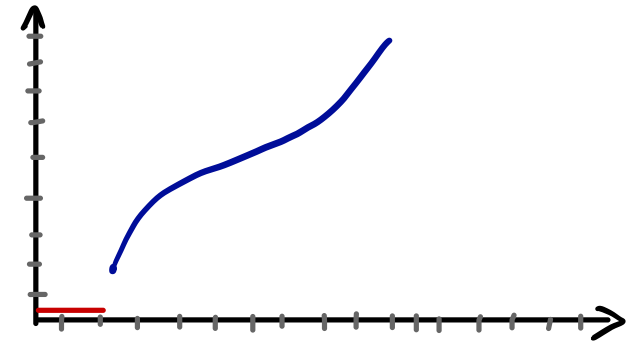
\includegraphics[scale=0.3]{20190411_073844099_iOS.png}
  		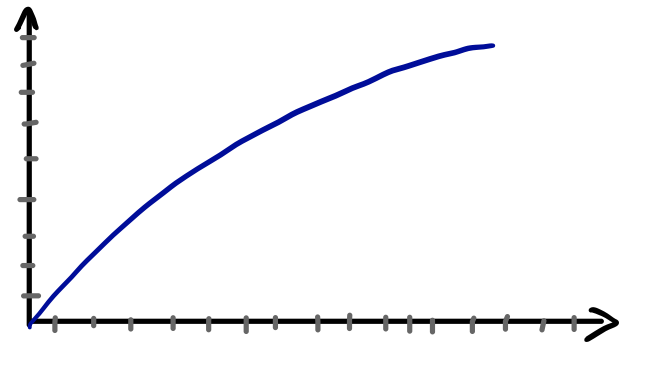
\includegraphics[scale=0.3]{20190411_074045495_iOS.png}
  		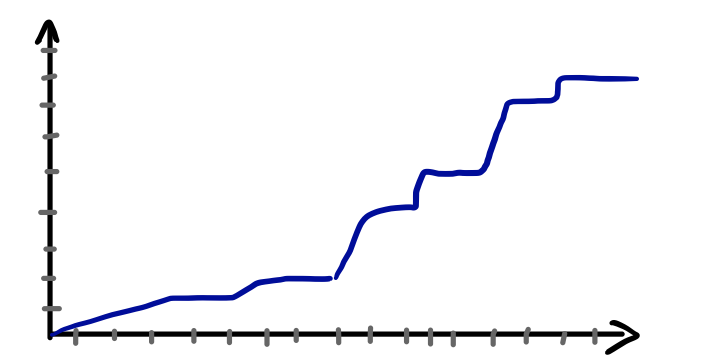
\includegraphics[scale=0.3]{20190411_074437642_iOS.png}
  		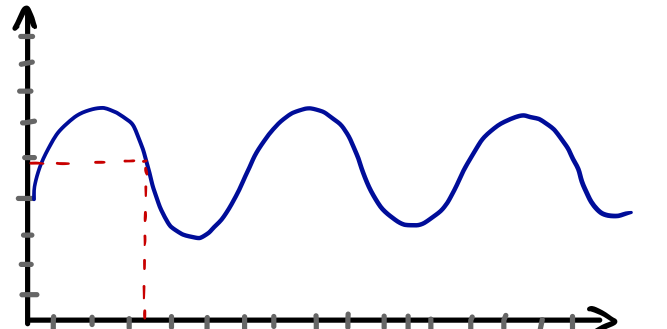
\includegraphics[scale=0.3]{20190411_074619898_iOS.png}\\
  	\textit{x-Achse = Zeit t; y-Achse= Position x}
  	\end{center}
 \subsection{1-dimensionale Bewegung}
 	\begin{center}
 			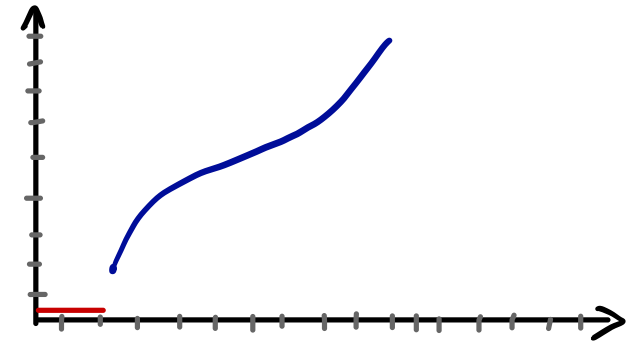
\includegraphics[scale=0.3]{20190411_073844099_iOS.png}
 	\end{center}
 \[ v = \frac{x_2 - x_1}{t_2 - t_1} = \frac{\Delta x}{\Delta t} \Leftrightarrow \lim_{\Delta t\to\ 0} \]
 Die Geschwindigkeit ist natürlich immer eine Durchschnittsangabe da es über eine gewisse Zeitspanne angeben wird. 
 
 \newpage
 \part{Vorlesung 3}
 			v = $\dot{x}$ \qquad v = $\frac{dx}{dt}$ \\
 			a = $\dot{v}$ = $\ddot{x}$ \qquad  a = $\frac{dv}{dt} = \frac{d^2x}{dt^2}$ \\
 			Mittelwerbeschleunigung = $\frac{\Delta x}{\Delta t} = \frac{\frac{x_4 - x_3}{t_4 - t_3} - \frac{x_2 - x_1}{t_2 - t_1}}{t_3 - t_1}$
  	\begin{center}
 	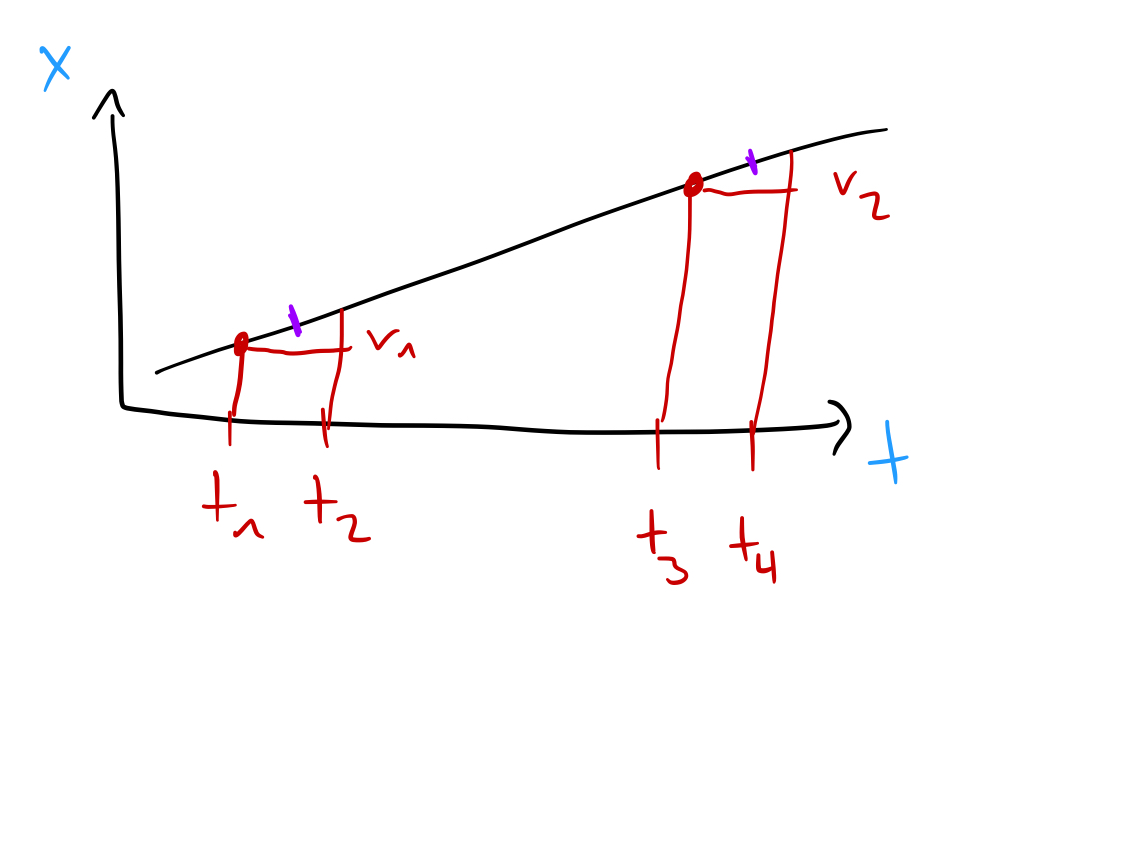
\includegraphics[scale=0.3]{IMG_EFF187166B54-1.jpeg}
 	\end{center}
 \[ v = \frac{dx}{dt} \rightarrow x_(t) = x_0 + \int_{t}^{t_0} v dt \]
\[ a = \frac{dv}{dt} \rightarrow v_(t)  = v_0 + \int_{t}^{t_0} a dt \]
	$x_(t)$ bei gegebenen $a(t)$ \\
		$x(t) = x_0 + \int_{t}^{t_0} (v_0 + \int_{t´´}^{t_0} a_(_t_) dt) dt´´$ \\
		
		$v(t)$ aus $a(x)$: \\
		v = $\frac{dx}{dt}$ \qquad dt = $\frac{dx}{v}$ \\
		a = $\frac{dv}{dt} $ \qquad dt = $\frac{dv}{a}$\\
		darauf ergibt sich $\frac{dx}{v} = \frac{dv}{a}$ $\Leftrightarrow \int_{v_1}^{v_0} v dv = \int_{x_1)}^{x_2} a_(x)dx$ durch weiteres umformen kommt man zum ausdruck: \\
		\[ \frac{1}{2} v^2 -\frac{1}{2} v_0^2 = \int_{x}^{x_0} a_(_x_)dx \]
 Wenn man nun die Masse mit einbezieht kommt man zur klassischen kinetischen Energie\\
  \[ \frac{1}{2} mv^2 - \frac{1}{2} mv^2 = \int_{x}^{x_0} a_(x) dx \]
  
  \section{3.3.4 Spezialfälle}
  	\subsection{Gleichförmige Bewegung}
  		a = 0  $\Leftrightarrow v = v_0$ \qquad $x_(_t_) = x_0 + v_0(t - t_0)$ \\
  		Also ist die Geschwindigkeit konstant 
	\subsection{konstante Beschleunigung}
			a = const \qquad $v = v_0 + a(t - t_0)$ \\
			$ x = x_0 + \int_{t_0}^{t} (v_0 + a(t - t_0))dt) \\
				= x_0 + \int_{t_0}^{t} v_0 dt + a \int_{t_0}^{t} (t - t_0) dt\\
				x = x_0 + v_0(t- t_0) + \frac{1}{2}a(t - t_0)^2 $ \\
			\textbf{Wahl des Koordinaten Systems:\\ t=0 und x=0}
			Gleichförmige Bewegung: $a = 0 ; v = v_0 \rightarrow x = v * t$ \\
			\textbf{konstante Beschleungung:} $a = const ; v = v_0 + a t ; x = vt + \frac{1}{2} at^2 $
\section{3.4 3-Dimensionale Bewegung (Vektoren)}
	  	\begin{center}
		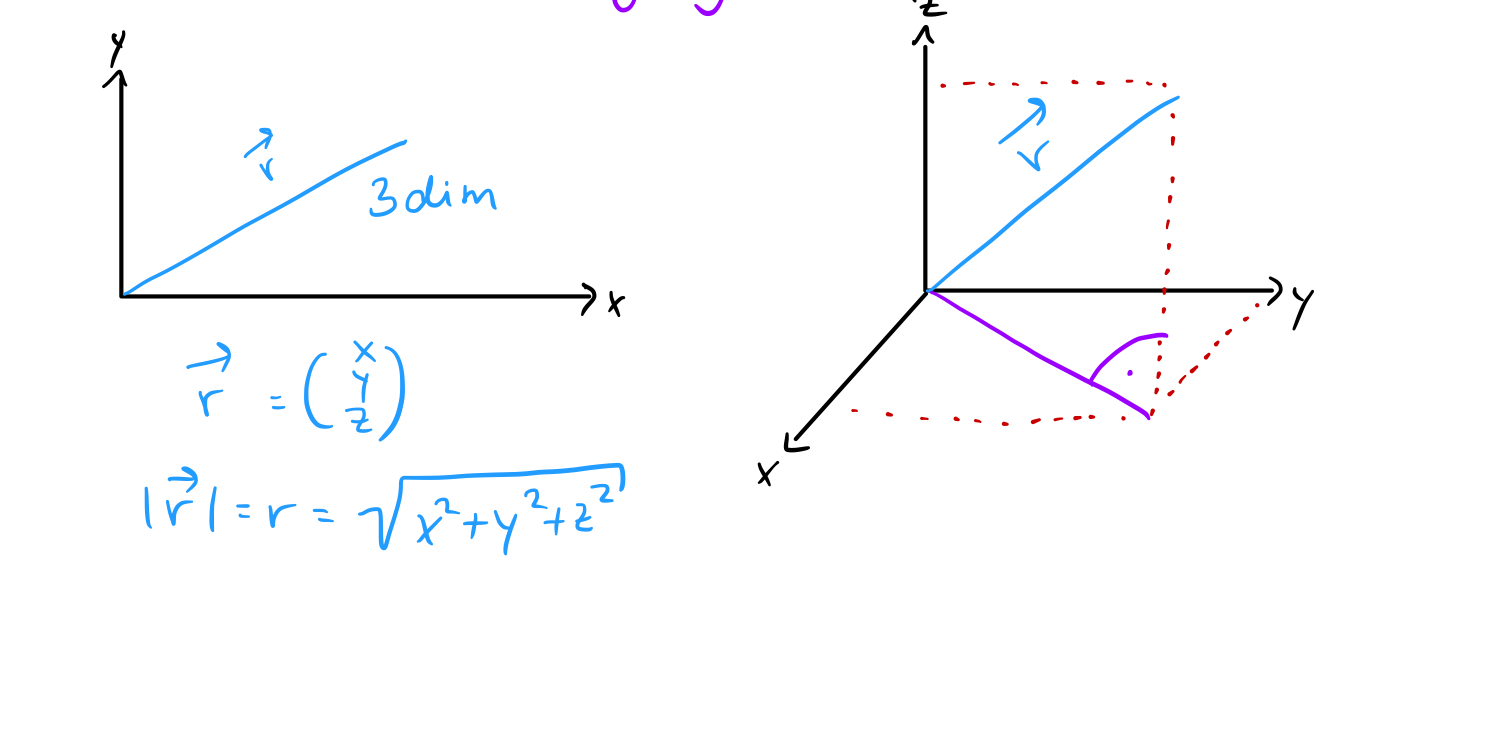
\includegraphics[scale=0.3]{IMG_8E3512F499A3-1.jpeg}
	\end{center}
	Sofern es keinen Vektorpfeil über einem Vektor gibt ist meist die Länge des Vektors gemeint\\
		$\vec{r} = \left(\begin{array}{cc}
		x \\
		y \\
		z
		\end{array} \right) $
		$\|\vec{r}\| = r = \sqrt{x^2 + y^2 + z^2}$ \\
		$\Leftrightarrow v_x = \frac{dx}{dt}$ \qquad $v_y = \frac{dy}{dt}$ \qquad $v_z = \frac{dz}{dt}$  \\
		\textbf{Beschleunigung} $a_x = \frac{d\vec{r}}{dt} 	\vec{a} = \frac{d\vec{v}}{dt}$

		\part{Vorlesung 4}
		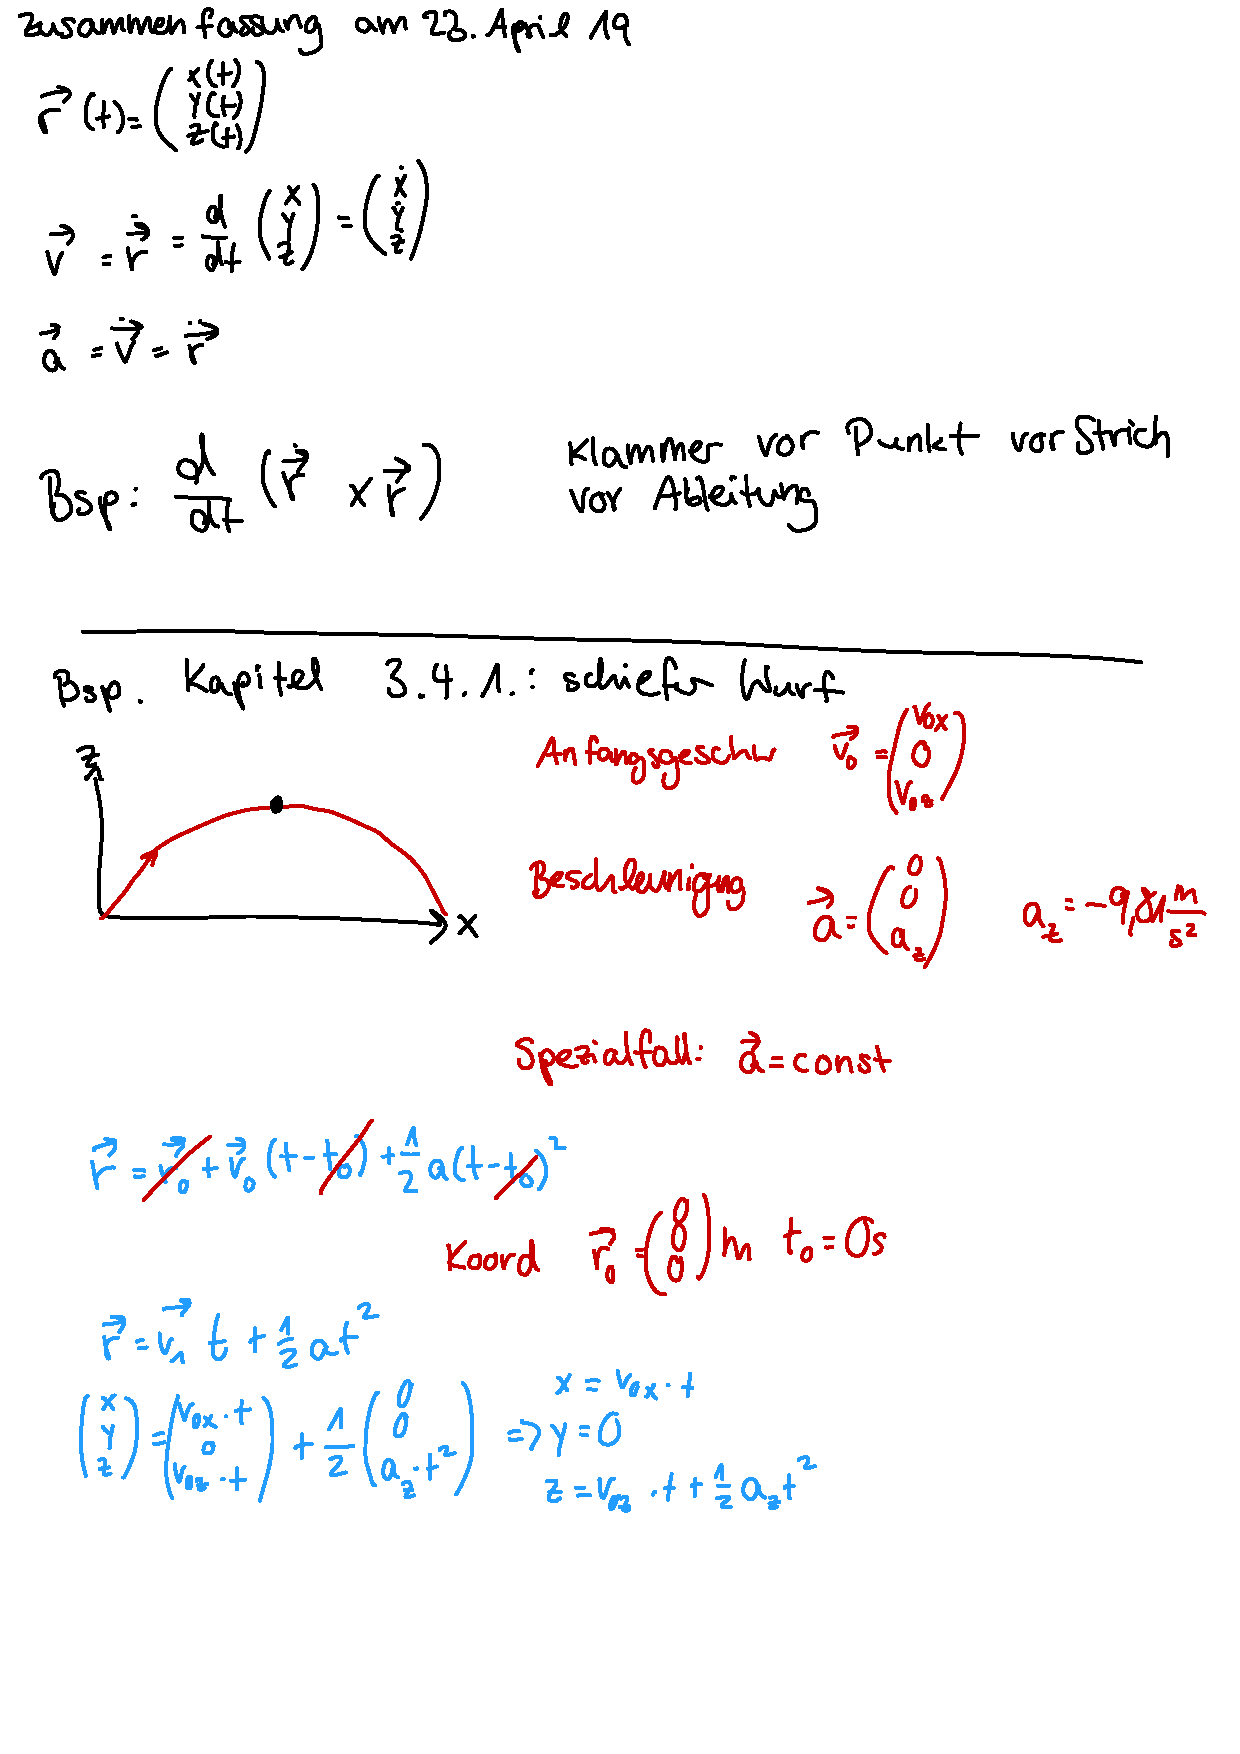
\includepdf[pages=-]{./images/PHY1-19.pdf}
		
		\part{Vorlesung 5}
			\section{Newton Axiome}
				\begin{itemize}
					\item \textbf{Trägheitsprinzip} Ein Körper bleibt in Ruhe oder gleichförmiger Bewegungn wenn keine resultierende äußere Kraft wirkt.
					\item \textbf{Aktionsprinzip} Ein Körper wird in Richtung der resultierenden äußeren Kraft beschleunigt und es gilt \[ \vec{F} = m * \vec{a} \], mit m = Masse des Körpers (Konstant) und $\vec{a}$ der resultierender Beschleunigungsvektor.\\ \textbf{$\vec{F} = \sum \vec{F}_i$}
					\item \textbf{actio = reactio} Die Kräfte treten immer Paarweise auf: Wenn der Körper A eine Kraft $\vec{F}^{(B)}_A$ auf einen Körper B ausübt, dann wirkt eine gleichgroße, aber entgegengesetzte gerichtete Kraft $\vec{F}^{(A)}_B$ von B auf A.\\
					\textbf{$\vec{F}^{(B)}_A =  - \vec{F}^{(A)}_B$}
				\end{itemize}
			\section{Inertialsysteme}
				In einem Intertialsystem gilt \textbf{$F= m * a$} in seiner reinsten Form. Es ist damit ein Bezugssystem, in welchem sich ein kräftefreier Körper gradlinig gleichförmig bewegt. Die \textbf{Newton´schen Axiome} gelten damit \textbf{nur in Intertialsystemen}\\
			\section{Gravitation}
				$ \vec{F}_{1 2} = G \frac{m_1 m_2}{r^2_{12}} \frac{\vec{r}_{21}}{\vec{r_{21}}} $
				$$\vec F_G=m\cdot\vec a_G$$
				$$F_G=m\cdot g$$
				\[ \vec F_{12}=-G\cdot\frac{m_1\cdot m_2}{r^2}\cdot\hat e_{21} \]
				$g$ ist ortsabh\ddot{a}ngig, $m$ ist eine intrinsische Eigenschaft.\\
				Dabei ist $ G = 6,67 * 10^{11} \frac{m^3}{kg s^2}$
					\subsection{Erdbeschleunigung}
				Die Annahme zum Ausrechnen der Erdbeschleunigung ist dass der Masseschwerpunkt im Mittelpunkt der Masse ist.\\
				\[ F_k = G \frac{M_E * m_k}{( r_E + h)12}  \quad h << r_E \]
				\[ F = G \frac{M_E}{r_E^2} * m_k  = g * m_k\]
				$\Rightarrow g = 9.81 \frac{m}{s^2}$\\
				Zum Momentananen Stand besprechen wir dabei nicht die Fluchtgeschwindigkeit. Diese wird aber zu einem späteren Zeitpunkt noch besprochen.\\
				Da die Erde eine so große Masse hat ist die beschleunigung dem entsprechend für uns klein $1 >> a$ wie aus $F = m * a$ folgt.
				\section{Tr\ddot{a}ge und schwere Masse}	
					$ \vec{F} = \frac{d\vec{p}}{dt} = \frac{d}{dt}(m_{tr\ddot{a}ge} * \vec{v}) $\\
					G mit $ \vec{F}_G  = G \frac{m_{1,schwer} * m_{2,schwer}}{r^2} * \frac{\vec{r}_{12}}{r_{12}} = g * m_{schwer}$\\
		Durch Experimente durchgeführt von \textbf{Eötvös }folge $m_{schwer} = m_{tr\ddot{a}ge}$ für alle Stoffe\\
		\[ G \frac{m_{tr\ddot{a}ge} * a}{\frac{m:E m_{schwer}}{r^2}} = konst = \frac{m_{tr\ddot{a}ge}}{m_{schwer} }= \frac{a * r^2}{G * m_E} \]
		\begin{figure}[htbp]
			\begin{minipage}[t]{6cm}
				\vspace{0pt}
				\centering
				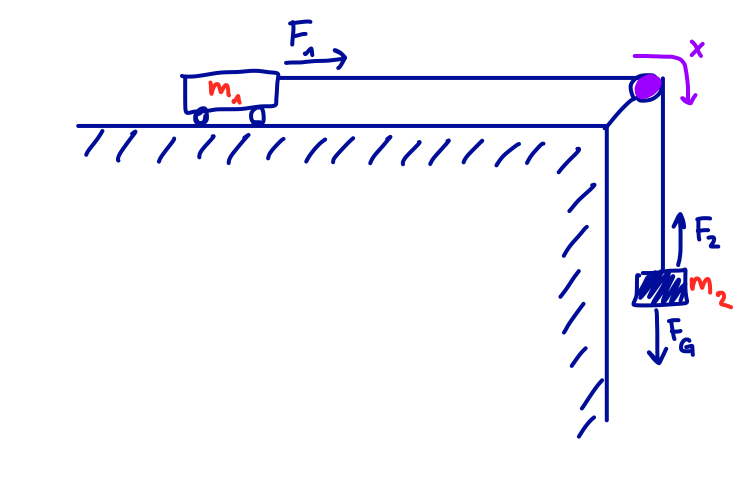
\includegraphics[scale=0.35]{IMG_E8A9C85E8431-1.jpeg}
			\end{minipage}
			\hfill
			\begin{minipage}[t]{6cm}
				\vspace{0pt}
				$ m_1 a_1 = F_1 $ (träge)\\
				$ m_2 a_2 = F_2 + F_G $ (träge)\\
				$ F_1 = - F_2 $\\
				Der Faden muss gespannt bleiben.\\
				$ a_1 = a_2 $\\
				$\Rightarrow m_1 a = - m_2 a $\\
				$ F_1 = -F_2 $\\
				$ m_{1, tr\ddot{a}ge} a_1 = F_1 = - F_2 = -(m_{2, tr\ddot{a}ge} a_2 -F_G) $\\
				mit $ F_G = -m_{2, schwer} g $\\
				$m_{1, tr\ddot{a}ge} a = - m_{2, tr\ddot{a}ge} - m_{2, schwer} g$	\ddot a
			\end{minipage}
		\end{figure}
		\[ a = \frac{m_{2, schwer}}{m_{1,tr\ddot{a}ge} + m_{2,tr\ddot{a}ge}} g \]
			\part{Vorlesung 6}
				Bei der Gravtitation gibt es einige Experimentelle Möglichkeiten die Gravitation zu veranchaulichen und zu beweisen. Im allgemeine gilt immer dass eine Schwere Masse immer eine Gravitation auf andere Objekte ausübt. Die Masse kann aber noch so gering sein und trotzdem wird dies einen unterschied im Gravitationsfeld machen, es wird nur für das Menschliche Auge nicht sichtbar sein da es viel größere Massen gibt.
				\section{Impulserhaltung}
					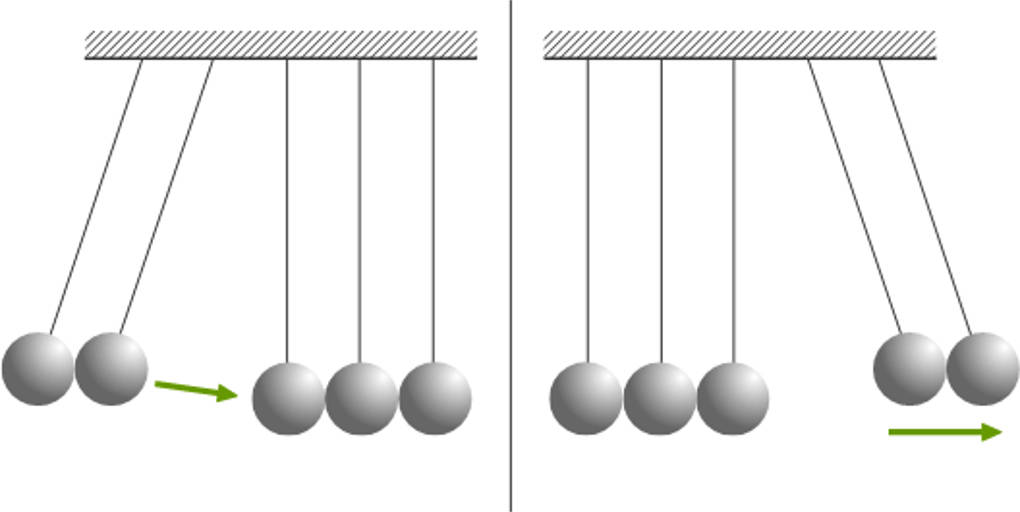
\includegraphics[scale= 0.4]{NewtonPendell.jpg} 
					$\sum \vec{F} = 0 \Rightarrow m_1,\vec{v}_1 + m_2 \vec{v}_2 = 0 = (m_1 + m_2 * \underbrace{\vec{v}_2}_{0}) $
			\subsection{Federn}
					\begin{figure}[htbp]
					\begin{minipage}[t]{6cm}
						\vspace{0pt}
						\centering
						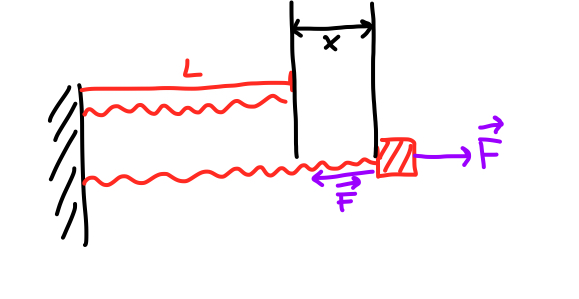
\includegraphics[scale=0.25]{IMG_13C2526BF067-1.jpeg}
					\end{minipage}
					\hfill
					\begin{minipage}[t]{6cm}
						\vspace{0pt}
						Ruhelage\\
						$ \vec{F} = - k \vec{x}$ (linear)\\
						$m \underbrace{\vec{a}}_{\ddot{x}} = \vec{F} = - k \vec{x}\\$
						$\ddot{x} + \frac{k}{m} \vec{x} = 0 $ Bewegungsgleichung\\
						\textbf{Differentialgleichung 2. Ordnung}
					\end{minipage}
				\end{figure}
			\subsubsection{Hook'sches Gesetz}
			$$F_x=-k_F\cdot\Delta x\quad\quad\Delta x\equiv x-x_0\equiv x$$
			$$\rightarrow\quad F_x=-k_F\cdot x$$
			Zuerst wird Arbeit an der Feder verrichtet (Verformung), dann verrichtet die Feder selbst Arbeit.
			$$W_{02}=\int_{x_0}^{x_2}F_x\Delta x=-\frac{1}{2}k_fx_2^2<0$$
			$$W_{20}=\int_{x_2}^{x_0}F_x\Delta x=\frac{1}{2}k_fx_2^2>0$$
			\subsubsection{Taylorentwicklung}
			In dem Fall gibt es auch das Beispiel der Taylorentwicklung der e-Funktion.
			$d_{(x)} \qquad d^\prime_{(x)}$\\
			$f(x) = f(x_0) + (x - x_0) f^\prime(x_0) + \frac{((x -x_0)^2}{2!} f^{\prime\prime}$\\
			$x_0 = 0$
			\[ f(x) = f(0) + (x-0) e^0 + \frac{(x-0)^2}{2!}e^0 + .... \\
			= \underbrace{1}_{\underbrace{Ruhelage}} + x + \frac{x^2}{2!} + \frac{x^3}{3!}+ .... \]
			\begin{center}
				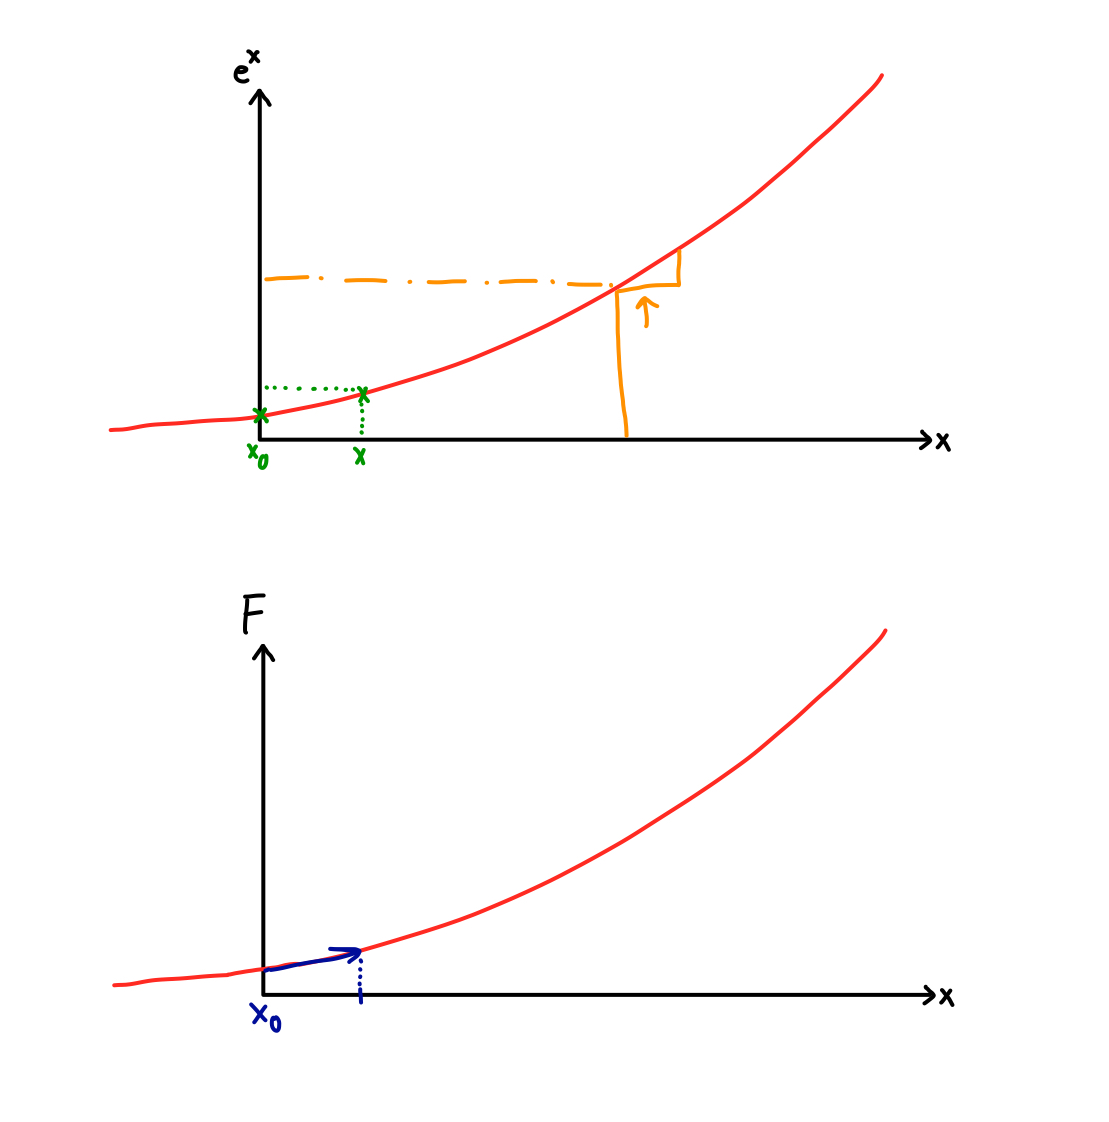
\includegraphics[scale=0.2]{IMG_94B96AE1BBE0-1.jpeg}
			\end{center}
		\begin{figure}[htbp]
			\begin{minipage}[t]{7cm}
				\vspace{0pt}
				\centering
				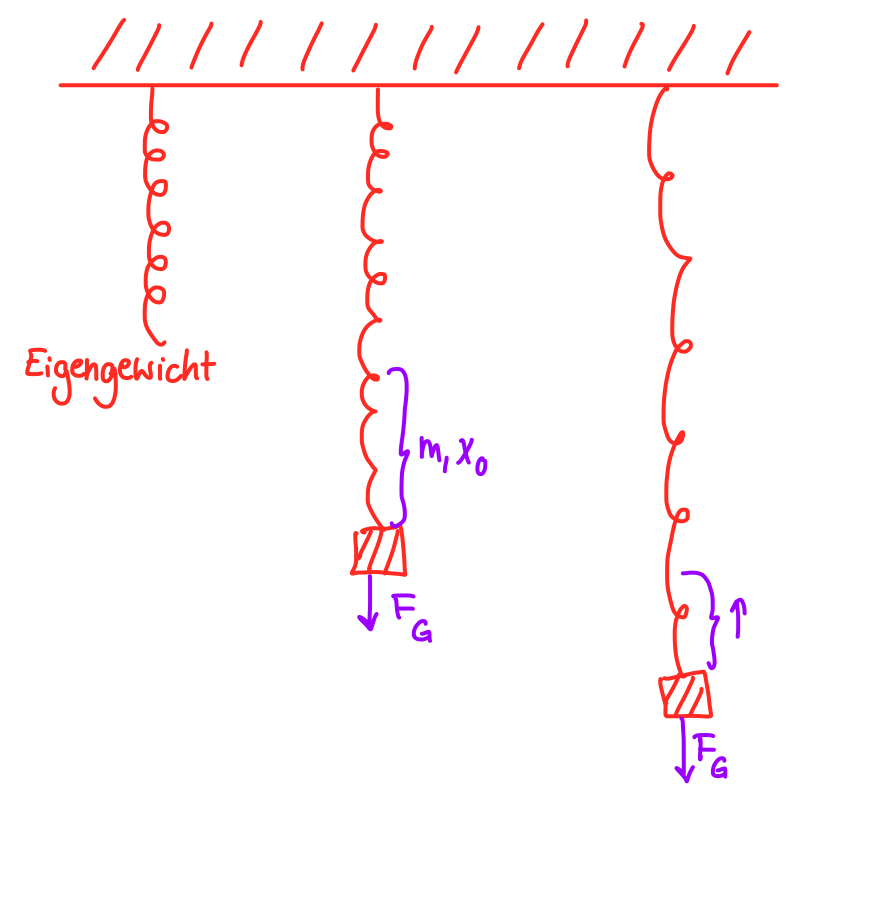
\includegraphics[scale=0.27]{IMG_EDD095C56715-1.jpeg}
			\end{minipage}
			\hfill
			\begin{minipage}[t]{7cm}
				\vspace{0pt}
				$F_G + F_{Feder} = mg - kx_0 \underbrace{=}_{(1} 0 \Rightarrow k$\\
				$ m \ddot{x} = mg - k \underbrace{(x_0 + x)}_{(1) einsetzen} $\\
				$ m \ddot{x} = kx $\\
				$ \ddot{x} \frac{k}{m}x $
			\end{minipage}
		\end{figure}
	\newpage
	\subsubsection{Seilspannung}
	\begin{center}
			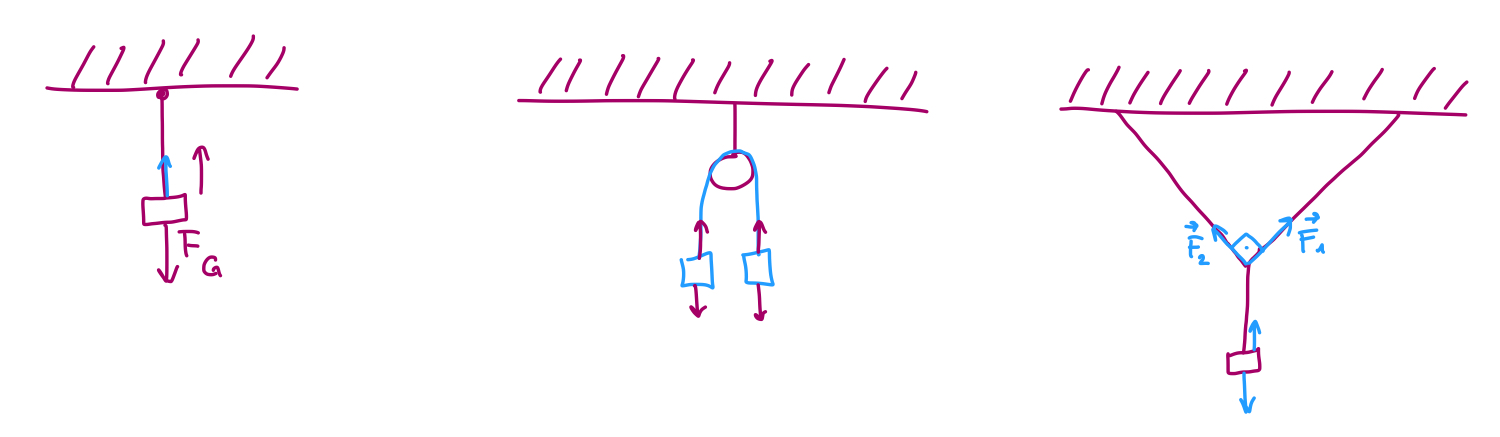
\includegraphics[scale=0.25]{IMG_64F74F51264B-1.jpeg}
	\end{center}
	$ m * a = \sum F = F_G + F_AS = 0 $
	$\sum \vec{F} = 0$\\
	$ - \vec{F}_G = \vec{F}_1 + \vec{F}_2 $\\
	$Notiz: \vec{F}_1 * \vec{F}_2 = |\vec{F}_1| * |\vec{F}_2| * cos \alpha$\\
	$ \vec{F}_G^2 = \vec{F}_1^2 + \vec{F}_2^2 + 2 \underbrace{\vec{F}_1 \vec{F}_2}_{= 0 \text{ wegen 90 grad}} $\\
	$S^2 = 4^2 + 3^2$
	\section{Reibung}
	\[ F_R = \mu * F \qquad \vec{F}_\sqcup \text{i st entgegen } \vec{v} \]
		\begin{center}
			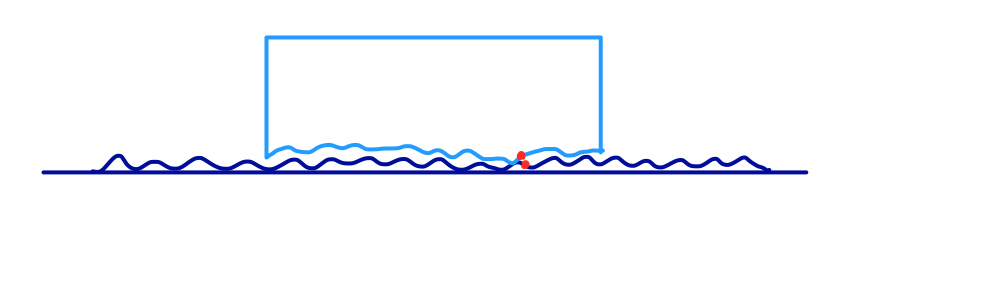
\includegraphics[scale=0.3]{IMG_60C9C3799F69-1.jpeg}
		\end{center}
	Reibungskraft: \\\begin{tabular}{|c|c|c|}
		\hline 
		\mu & Haft & Gleit \\ 
		\hline 
		Stahl -Stahl & 0,75 & 0,57 \\ 
		\hline 
		Teflon - Teflon & 0,04 & 0,03 \\ 
		\hline 
	\end{tabular} 
	\subsubsection{Stokes Reibung}
		Reibung im Wasser
		\begin{figure}[htbp]
			\begin{minipage}[t]{7cm}
				\vspace{0pt}
				\centering
				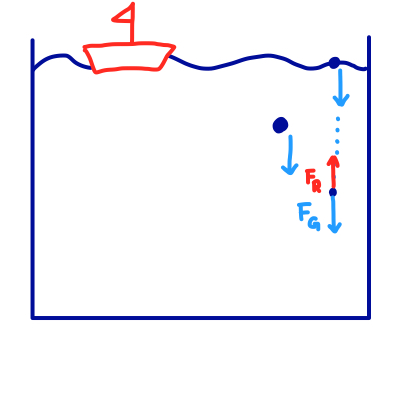
\includegraphics[scale=0.27]{IMG_972B7A9BCF52-1.jpeg}
			\end{minipage}
			\hfill
			\begin{minipage}[t]{7cm}
				\vspace{0pt}
				$ F_R = 6 \pi * r \mu * v $
				$ \Rightarrow $ Viskosität\\
				$ |F_R| = |F_G| \Rightarrow mg = 6 \pi r \mu v $\\
				$ \Righarrow  v = konst $\\
				solange v klein ist
			\end{minipage}
		\end{figure}
		\subsubsection{Newton-Reibung}
			$ F_R = \frac{1}{2} \underbrace{a_w}_{\text{spezifische Luftwiederstand |}}  \underbrace{\rho}_{\text{Dichte der Luft}} A v^2 $
			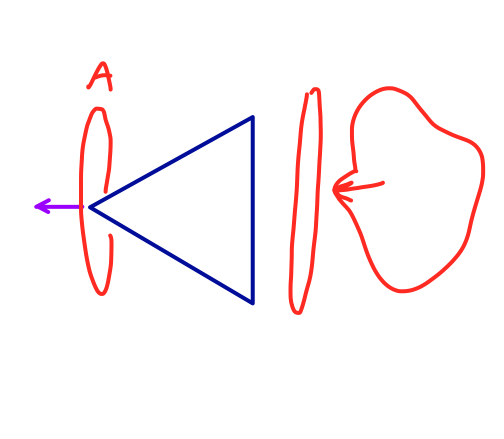
\includegraphics[scale=0.3]{IMG_7A852B76F915-1.jpeg}
		\part{Vorlesung 8}
			\subsection{Wiederholung}
				Angenommen man habe eine Senke und ein Auto welcher hinterrutscht. Man hat also drei Kräfte die Aufrreten. Diese Wären die Gewichtskraft, die Normalkraft und die Reibung(Haftreibung). Dazu gilt wenn die nicht negative Kraft größer ist als die Haftreibung dann herscht beschleunigung.
				\[ F_{Haft} = \mu F_N \]
				\[ \text{Gleitreibung } F_{Gleit} = \mu_G F_N \]
		\section{Schwingungen}
			\subsection{Harmonischer Oszilator}
				Wenn man eine Feder hat und an dieser irgendeine Masse m hängt, gibt es logischerweise eine Auslenkung an der Feder. Damit wirkt natürlich eine Kraft nach oben und die Federkraft nach unten.
				\[ m \ddot{x} = F = - kx  \]
			Und nun zur Bewegungsgleichung des Harminischen Oszilator. Dieser Fall lässt sich auf sehr viele Beispiele  anwenden. 
			\[ \ddot{x} + \frac{k}{m}x = 0 \]
				\subsubsection{Pendel}
					Man nehme ein Pendel in einer Ruhelage und ein weiteres Pendel welches dem anderen Pendel volkommen gleicht. Das zweite Pendel unterscheidet sich lediglich durch die auslenkung des Pendels um den Winkel $\varphi$. \\ 
					Die \textbf{Masse} ist bei einem Pendel volkommen egal da nur die Gewichtskraft auf die Masse des Pendels wirkt.\\
					Wir sagen nun, dass wir bei dem zweiten Pendel noch zusätzlich eine Tangentialkraft haben welche logischerweise in Richtung des Ruhelage zeigt.
					\[ F_T = -F_G \cdot sin \varphi = -mg \cdot sin \varpi \]
					Nun nutzen wir die defnition des Bogenmaßes um folgende Gleichung daraus zubekommen.
					\[ \underbrace{x_T}_{Umfang aller Bahnen} = \underbrace{l}_{Radius} \cdot \underbrace{\varphi }_{Winkel} \]
					Also \\
					$\ddot{x}_T = l \ddot{\varphi}$
					\[ F_t = m_{Tr\ddot{a}ge} \cdot \underbrace{a_T}_{\ddot{x}_T}  \Rightarrow m_{g} \cdot g \cdot sin \varphi = m_T \cdot l \ddot{\varphi} \]
					$ \Rightarrow$
					\begin{tcolorbox}
						\begin{align}
							\ddot{\varphi} + \frac{g}{l}sin \varphi = 0
						\end{align}
					\end{tcolorbox}
				\textbf{Nährung dazu:} $sin \varphi \approx \varphi$ in Bogenmaß für kleine $\varphi$
				\begin{tcolorbox}
					Ein Praktischer Exkurs:
					\begin{align}
						\varphi_{\text{in Grad}} = \varphi_{Bogenmaß} \cdot \frac{360^\circ}{2\pi}
					\end{align}
				\end{tcolorbox}
			\subsection{allgemeine Lösung harmonischer Oszilator:}
				Feder: $w^2 = \frac{k}{m}$ \qquad
				Pendel $ w^2 = \frac{g}{l} $\\\\
				\textbf{Bewegungsgleichung}: $ \ddot{y}_{(t)} + w^2 y_{(t)} = 0$
				Da wir nun eine Differentialgleichung haben brauchen wir nun einen Ansatz den wir raten müssen.
				\[ \dot{y}_{(t)} =\ A \cdot\ sin (w\cdot t) + B\ \cdot\ cos(w \cdot t)  \]
				$\dot{y} = w \cdot A \cdot cos(wt)\quad  - w \cdot B \cdot sin (wt)$\\
				$\ddot{y} = -w^2 \cdot A \cdot sin (wt)- w^2\cdot B\cdot cos(wt)} $\\
				$ \ddot{y}_{(t)} - w^2 y_{(t)} $\\
				\subsubsection{Anfangsbedingungen}
				\begin{itemize}
					\item \textbf{1. Fall:} $y_{(0) = y_{{0}}} = B $\\
							\qquad $\dot{y}_{(0)} = 0 = w A$\\
								\qquad \qquad $\Rightarrow A = 0$
						$y_{(t)} = y_0 \cdot cos (w t )$
					\item \textbf{2. Fall} $ y_{{0}} = 0 = B $\\
					\qquad $\dot{y}_{(0)} = v_0 = w \cdot A$\\
						\qquad \qquad $ \Rightarrow A = \frac{v_0}{w} $\\
						Die beiden letzen Zeilen zusammen ergibt dann:\\
						$y_{(0)} = \frac{v_0}{w} sin (wt) $
					\item \textbf{Alternative:}\\
						\qquad $y_{(0)} = C \cdot (wt + \varphi_0) $\\
						Wir nutzen nun die die Additionstheoreme.\\
						\qquad $C \cdot sin(wt) \cdot cos \varphi_0  $\\
						\qquad $C \cdot cos (wt) \cdot sin \varphi_0$\\
					\end{itemize}
						$ = \underbrace{C \cdot cos \varphi_0}_{A} \cdot sin (wt) + \underbrace{C \cdot sin \varphi_0}_{B} \cdot cos (wt) $
						\[ \text{wir setzen die Dimension } [w] = \frac{1}{s} \text{ also die Kreisfrequenz} \]
						$sin(wt) $\\
						Ich überspringe einfach mal die weitere Herleitung:
						\[ w = \frac{2 \pi}{T} \qquad w= \sqrt{\frac{g}{l}} \text{ bzw. } \sqrt{\frac{k}{m}} \qquad [w] = \left( \frac{m}{s^2 m} \right)^\frac{1}{2} = \frac{1}{s} \]
					\section{4.7 Variable Masse}
						\begin{align*}
							\frac{d \vec{p}}{dt} &= \vec{F} \Rightarrow \vec{p} = \vec{F} dt\\
							 &= \int _{p_0}^{p(t)} d\vec{p} = \int_{t_0}^{t} \vec{F} dt\\
							&=  p_{(t)} - p_0 = \underbrace{\int_{t_0}^{t} \vec{F} dt}_{\text{Kraftstoß}} 
						\end{align*}
						\subsection{Bsp. inelastischer Stoß}
							\[ v^\prime =\frac{m_1}{m_1 + m_2} v_2 \]
					\part{Vorlesung 9}
						\textbf{Wiederholung}\\
							Man stelle sich vor man habe eine Kraft die proportional zu einer Auslenkung von der Ruhelage ist.
							So hat man die Differentialgleichung einer Schwingung: $ \ddot{x} + w^2 x = 0 $
							\[ x_{(t)} = A \cdot sin (wt) + B \cdot cos (wt) \] 
					\subsection{Rakete}
						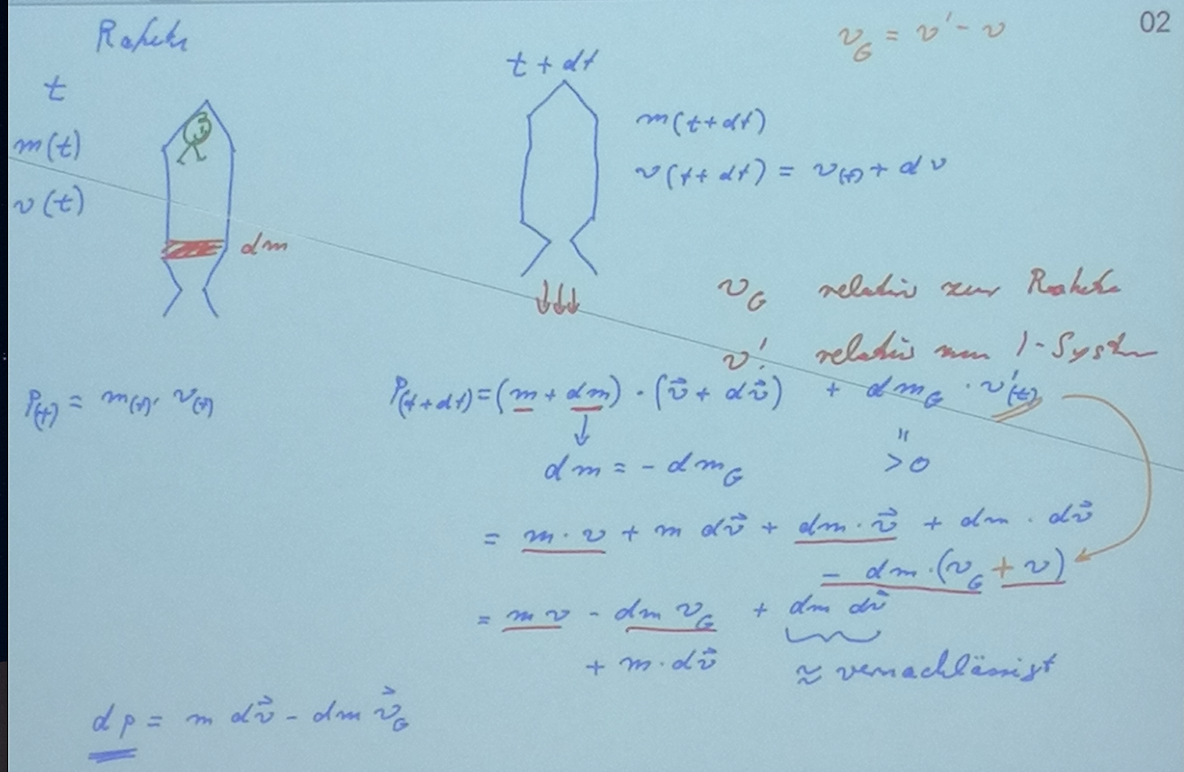
\includegraphics[scale=0.60]{Rakete.png}\\
						\textbf{Äußere Kraft:}\\
						F = $\frac{d \vec{p}}{dt} = m \frac{d \vec{v}}{dt} - \frac{dm }{dt} \vec{v}_G$
						\begin{tcolorbox}
							\begin{align}
								-mg = m \cdot \dot{\vec{v}} - \dot{m} \cdot \vec{v}_G
							\end{align}
							Wird nun mit $ \frac{dt}{m} $ multipliziert\\
							Das ganze muss immer größer 0 sein. 
						\end{tcolorbox}
					\[\underbrace{ |\vec{v}_G| \cdot |\frac{dm}{dt}}_{Schubkraft} \text{ kleiner als } mg \]
					\subsubsection{Lösung}
						\[ -\sum_{t_0}^{t} g \cdot dt = \sum_{\vec{v}_0}^{\vec{v}_{(t)}} d\vec{v} - \sum_{m_{(t)}}^{m_0} \frac{dm}{m} \cdot \vec{v}_G = \]
					\begin{tcolorbox}
						\begin{align}
						\vec{v}_{(t)} = \vec{v}_0 - g(t-t_0) + |\vec{v}_G| \cdot ln \frac{m_0}{m_{(t)}}
						\end{align}
					\end{tcolorbox}
				\section{4.8 Energie}
					\subsection{Arbeit}
						Wir gucken uns zunächst die Arbeit für ein sehr kleines Stück eines Weges an.
						\[ dW = \vec{F} \cdot d \vec{r} = F_r \cdot |d\vec{r}| \]
						$ \int dW = \sum \vec{F} \cdot \vec{v} dt $ \qquad \qquad dabei ist $d\vec{r} = 
						\left(\begin{array}{c}
						dx \\ 
						dy \\ 
						dz
						\end{array} \right)$\\
						und $ \vec{v} = \frac{d\vec{r}}{dt} $\\\\
						Es gibt aber noch die möglichkeit, die häufig auftritt und die Rechnung erheblich vereinfacht ist, dass:\\
						$ \text{ falls } \alpha = const $\\
						$ w = cos \alpha \int |\vec{F}| ds $
							\subsubsection{Beispiel: Der Freie Fall}
							Wir haben damit einen Punkt A und einen Punkt B wobei A höher liegt als B. die Distanz zwischen den beiden Punkten bezeichnen wir mit $h$.
							\[ \vec{r}_A \left(\begin{array}{c}
							0 \\ 
							0 \\ 
							h
							\end{array} \right) \quad \vec{r}_B \left(\begin{array}{c}
							0 \\ 
							0 \\ 
							0
							\end{array} \right) \quad \left(\begin{array}{c}
							0 \\ 
							0 \\ 
							dz
							\end{array} \right) \quad \vec{F} = \left(\begin{array}{c}
							0 \\ 
							0 \\ 
							-mg
							\end{array} \right) \]
							$ \Rightarrow W = \int_{\vec{r}_A}^{\vec{r}_0} \vec{F} d\vec{r} = - \int_{h}^{h} m\cdot g dz = - m\cdot g\cdot (0-h) = m \cdot g \cdot h $
				\subsubsection{Bsp: Feder}
					$ F = - kx $\\
					$ \left[ W = \int \vec{F} d\vec{r} = \int_{x_0}^{0} F dx = -k \frac{x^2}{2} \right|^0_x_0  = \frac{1}{2} k x^2 \right]$
				\subsubsection{Konstante Kraft}
					$\vec{F} = konst$\\
					\begin{itemize}
						\item W = $\int_{A}^{B} \vec{F} d\vec{r} = \vec{F} \int_{A}^{B} d\vec{r} = \vec{F}( \vec{r}_B - \vec{r}_A )$\\
						$r_B$ ist dabei der Endpunkt und logischerweise ist $r_A$ dann der Anfangspunkt.
					\end{itemize}
			\subsection{Konservative Kräfte}
				Fast alle Kräfte in der Natur sind konservative Kräfte.
				\begin{itemize}
						\item $\vec{F}$ konstant
						\item $\vec{F}$ Zentralkraft (F hängt nur von r ab also vom Zentrum der Kraft)
				\end{itemize}
				Es ist keine konservative Kraft, wenn diese von der Zeit oder von der Geschwindigkeit abhängt. Ein Beispiel für eine Kraft die von der Geschwindigkeit abhängt wäre beispielsweise die Reibung.\\\\
				\textbf{Eine konservative Kraft W ist unabhängig vom Weg}
				\subsubsection{Das gechlossendes Wegintegral}
					$ \oint \vec{F} d\vec{r} = 0 $ für konservative Kräfte
\part{Vorlesung 10}
	\textbf{Arbeit:}
	\begin{align*}
		dW &= \vec{F} d\vec{s}\\
		W &= \int \vec{F} d\vec{s} = \int \vec{F} \vec{v} dt
	\end{align*}
		\section{4.9 Potentielle Energie & Potential}
			Wenn wir einen Weg haben mit einem start und einem Endpunkt, dann ist der Weg als Arbeit definiert.\\
			So haben sowohl anfangs als auch endpunkt eine Potentielle Energie.
			\begin{align*}
				W = \int_{A}^{B} \vec{F} d\vec{r} = E_{Pot, A} - E_{Pot, B}
			\end{align*}
	Dazu machen wir jetzt noch ein Paar Beispiele. Was man noch anmerken kann ist, dass Potentielle Energie nur für konservative Kräfte formuliert ist, durch einfache überlegungen dürfte dies auch klar werden.\\
	Wie bereits bekannt ist die Potentielle Energie:
	\[ E_{Pot} = m \cdot g \cdot h \]
	\subsection{Beispiel}
		\begin{align*}
			E_{Pot(h)} - \underbrace{E_{Pot, (0)}} }_{ E_{Pot(h=0)= 0} } = W = m\cdot g \cdot h
		\end{align*}
		\subsection{Gravitation}
		\begin{align*}
			\vec{F} &= -G \frac{m_1 m_2}{r_{12}^2} \frac{\vec{r}_{12}}{r_{12}}\\
			E_{pot}(r = 0) - E_{Pot}(r) &= - \int G\frac{m_1 m_2}{r^2}dr = G \frac{m_1 m_2}{r}
		\end{align*}
		\begin{theorem}
			\[E_{Pot (r)}= - G \frac{m_1 m_2}{r} \]
		\end{theorem}
		Die Potentielle Energie ist also immer negativ für eine \textbf{Anziehende Kraft}.
		\begin{theorem}
			\[V_{(r)} = - G \frac{m_1}{r} \]
		\end{theorem}
	Nun stellen wir uns die Frage wie man das ganze Rückwärts machen würde oder ob das überhaupt möglich ist. Die Antwort ist ja, es geht.
	\subsection{Von Potentieller Energie auf Engergie schließen}
		\[ \vec{F} \rightarrow E_{pot} \]
		$E_{pot, B} - E_{pot-A} = \int_{A}^{B} F_x dx  $\\
		$ dF_{pot} = - F_x dx $\\
		$ F_x= -\frac{dE_{pot}}{dx}$
		\begin{theorem}
			\begin{align*}
				\vec{F}= - \nabla E_{pot(\vec{r}) }
			\end{align*}
			Ableitung des Potentials ist die Kraft.
		\end{theorem}
	\subsection{kinetische Energie}
		\begin{theorem}
		\begin{align*}
			\frac{1}{2}m v ^2
		\end{align*}
				Wie bereits bekannt ist wird so die Potentielle Energie definiert. Es gibt viele verschiedene Möglichkeiten dies zu beweisen. Folgendes st eine Möglichkeit die wir in der Vorlesung genutzt haben.
		\end{theorem}
			\begin{proof}
				I\begin{align*}
				F_T = m \frac{dv}{dt}\\
				\vec{F} d\vec{r} = F_T ds &= m \frac{dv}{dt} ds\\
				&= m = \frac{ds}{dt}dv\\
				&= m \cdot v dv\\
				W = \int_{A}^{B} \vec{F} d\vec{r} = \int_{V_A}^{V_B} m \cdot v dv = \frac{1}{2}mv^2 |_{V_a}^V_B\\
				= \frac{1}{2} m \left( \vec{v}_B^2 - \vec{v}_A^2 \right)\\
				E_{kin} = \frac{1}{2} m \vec{v}^2 = \frac{\vec{p}^2}{2m}\\
				W = E_{kin, B}E_{kin, A}
				\end{align*}
			\end{proof}
 			\subsection{Energieerhaltung}
 				$ W = E_{kin, B} - E_{kin, A} $\\
 			$	W = E_{pot, A} - E_{pot, B} $
 			\begin{theorem}
 				\begin{align*}
 					E := E_{pot, A} + E_{pot, A} = E_{pot, B} + E_{pot, B}
 				\end{align*}
 			\end{theorem}
 		Ein Gutes Beispiel dafür wäre mal wieder eine Feder.
		\subsection{4.10 Drehbewegung}
			"Drehmoment ist das was das Drehmoment ändert."
	\begin{align*}
		\vec{r}_{(t)} = R \left( \begin{matrix}
		cos (wt)\\
		sin(wt)
		\end{matrix} \right)
	\end{align*}
	Damit definieren wir nun die Winkelgeschwindigkeit:\\
	\begin{theorem}
		$w = \dot{\varphi}$\\
		Die Winkelgeschwindkeit sagt also aus wie viel sich der Winkel ändert
	\end{theorem}
\begin{align*}
		\vec{v}_{(t)} = \dot{\vec{r}} = \dot{\varphi} R \begin{matrix}
		-sin \varphi\\
		cos \varphi
		\end{matrix}\\
		\vec{v} = \vec{w} \times \vec{r}\\
		\vec{a} = \dot{\vec{v}} = \ddot{\varphi} R \begin{matrix}
		-sin \varphi\\
		cos \varphi
		\end{matrix} + \underbrace{\dot{\varphi}^2}_{w^2} R \underbrace{\left(\begin{matrix}
		- cos \varphi\\
		- sin \varphi
		\end{matrix}\right)}_{-\vec{v}}\\
	=\vec{a} = \underbrace{\dot{w} R \vec{e}_v}_{ \text{erhöht Rotationsgeschwindigkeit} } - \underbrace{w^2 \cdot r}_{ \text{Zentripetalkraft nach innen}}
\end{align*}
	\part{Vorlesung 11}
		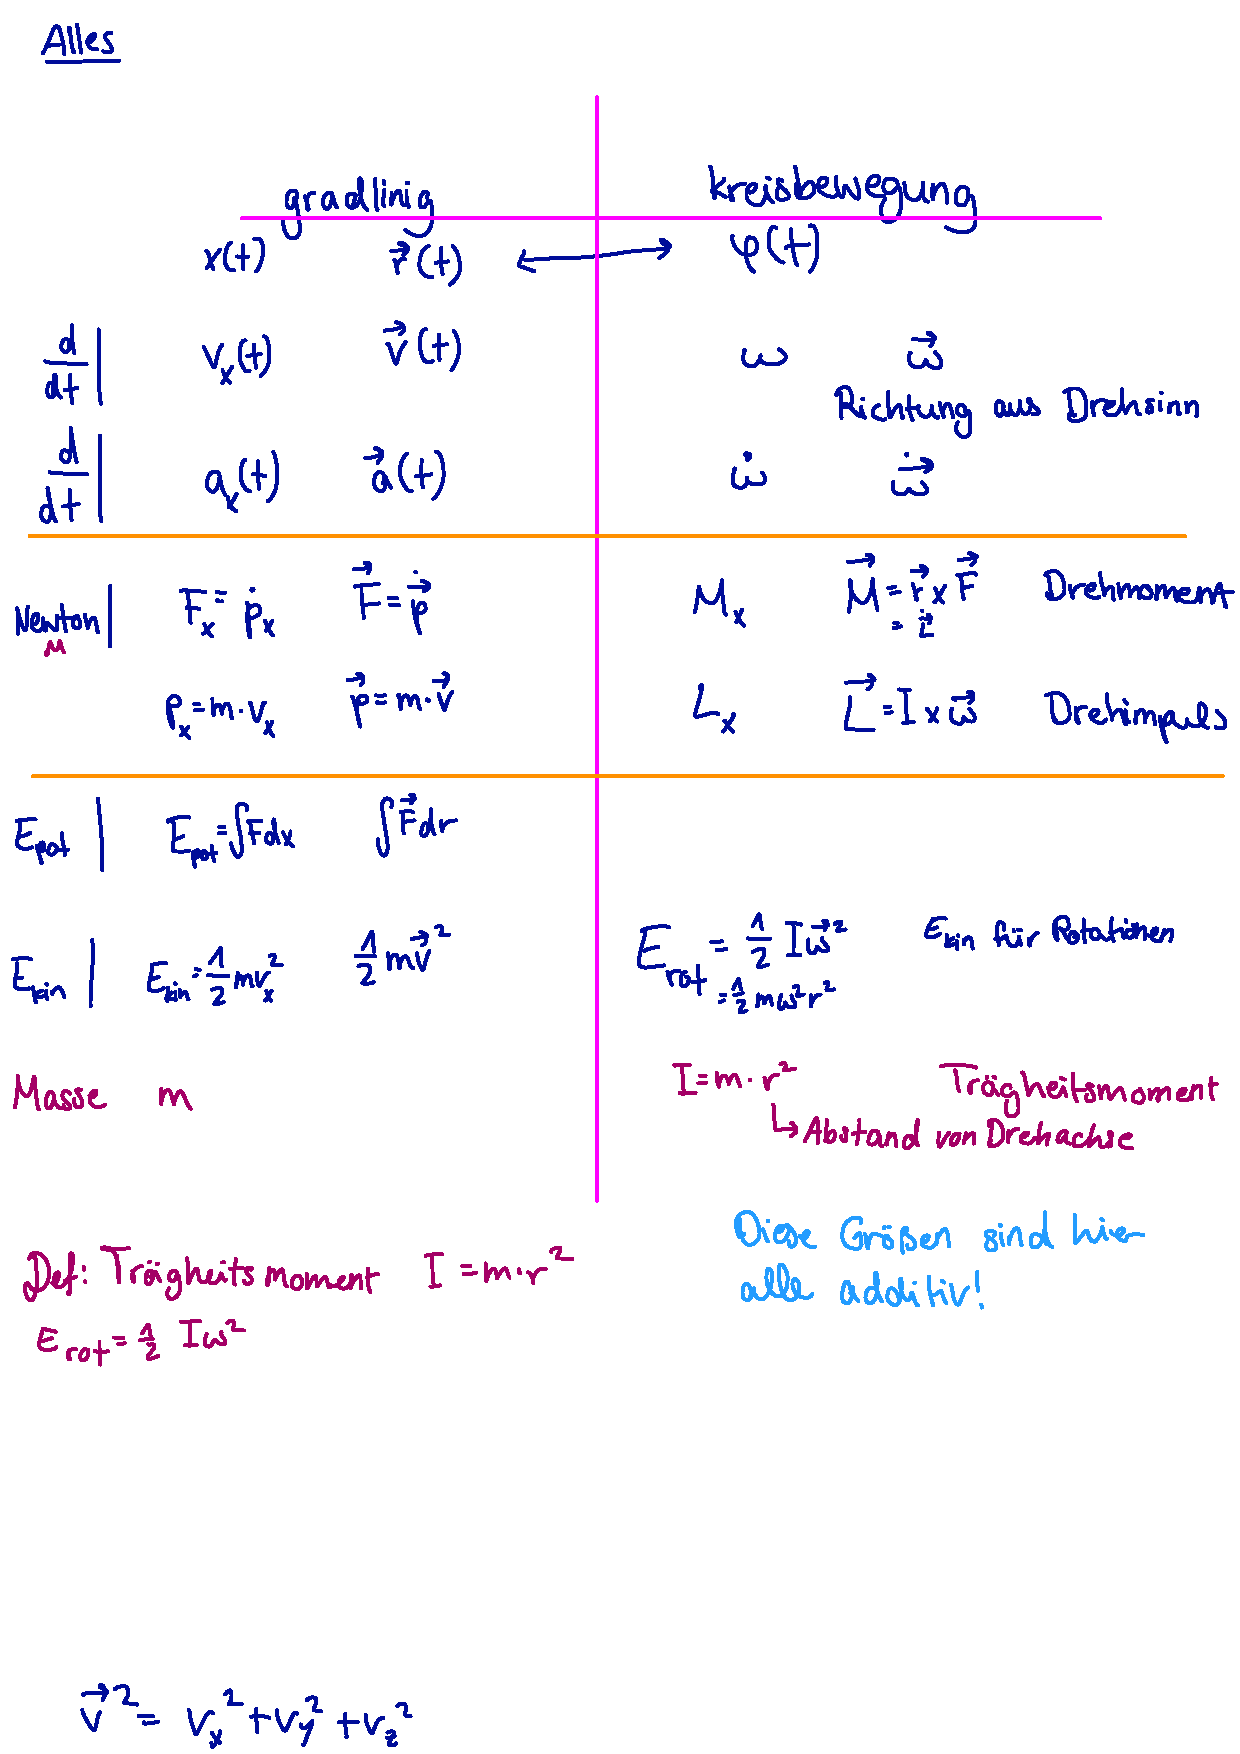
\includepdf[pages=-]{./images/Vorlesung12.pdf}
	\part{Vorlesung 12}
		\subsection{4.11 Drehmomente}
			\[ \vec{M} = \vec{r} \times \vec{F} \]
			\[ \dot{\vec{L}} = \vec{M} \qquad \vec{L} = \vec{r} \times \vec{p}  \]
		\section{Scheinkräfte}
			Es gibt verschiedene möglichkeiten sich zu bewegen. Wir nehmen uns nun die Gradlinige Beschleunigung und die Rotation. Dazu haben wir jetzt noch ein Initialsystem $S$ mit der Kraft $\vec{F}$ und der beschleunigung $\vec{a}$. zu diesen größen gibt es dann noch jeweils die $^\prime$ komponente die für das Relativistisch Beschleunigte System steht..\\\\
			\textbf{Gradlinige Beschleunigung:}\\
			\[ v_{(t)} = const \quad\vec{r}^\prime = \vec{r} - v \]
			\[ \vec{v}^\prime =\vec{v} - v \Rightarrow \vec{a}^\prime = \vec{a} \]
			$ \vec{V}_{(r)} = \text{ nicht konstant} $
			\[ \vec{a}^\prime = \vec{a} - \vec{A} \text{ gradlinige Beschleunigung } \qquad m \vec{a}^\prime = m \vec{a} - m \vec{A} \]
			\[ \vec{F}^\prime = \vec{F} - \underbrace{m \vec{A}}_{\text{Trägheitskraft}}  \]
		\textbf{Rotation}\\
		\[ \vec{F}^\prime = \vec{F} - \underbrace{2m \vec{w} \times \vec{v}^\prime}_{\text{Corioliskraft}} - \underbrace{m \vec{w} \times (w \times \vec{r}^\prime)}_{\text{Flächenkraft}} \]
	\section{6 Zweiteilchen Systeme}
		\subsection{Schwerpunktsystem und Relativsystem}
			^\begin{itemize}
					\item Erde $-$ Mond 
					\item H \quad proton $+$ elektron
					\item $O_2$ \quad O + O
					\item Feder von box $1$ zu box $2$
				\end{itemize}
		$\vec{F}_{21} = - \vec{F}_{12} \Leftarrow$ innen\\
		$ \vec{F}_1 , \vec{F}_2 \Leftarrow$ äußere\\
		$ m_1 \ddot{\vec{r}}_1 = \vec{F}_{12} + \vec{F}_1 $\\
		$ m_2 \ddot{\vec{r}}_2 = \vec{F}_{12} + \vec{F}_2 $
		\subsection{Rechnung}
		\begin{center}
			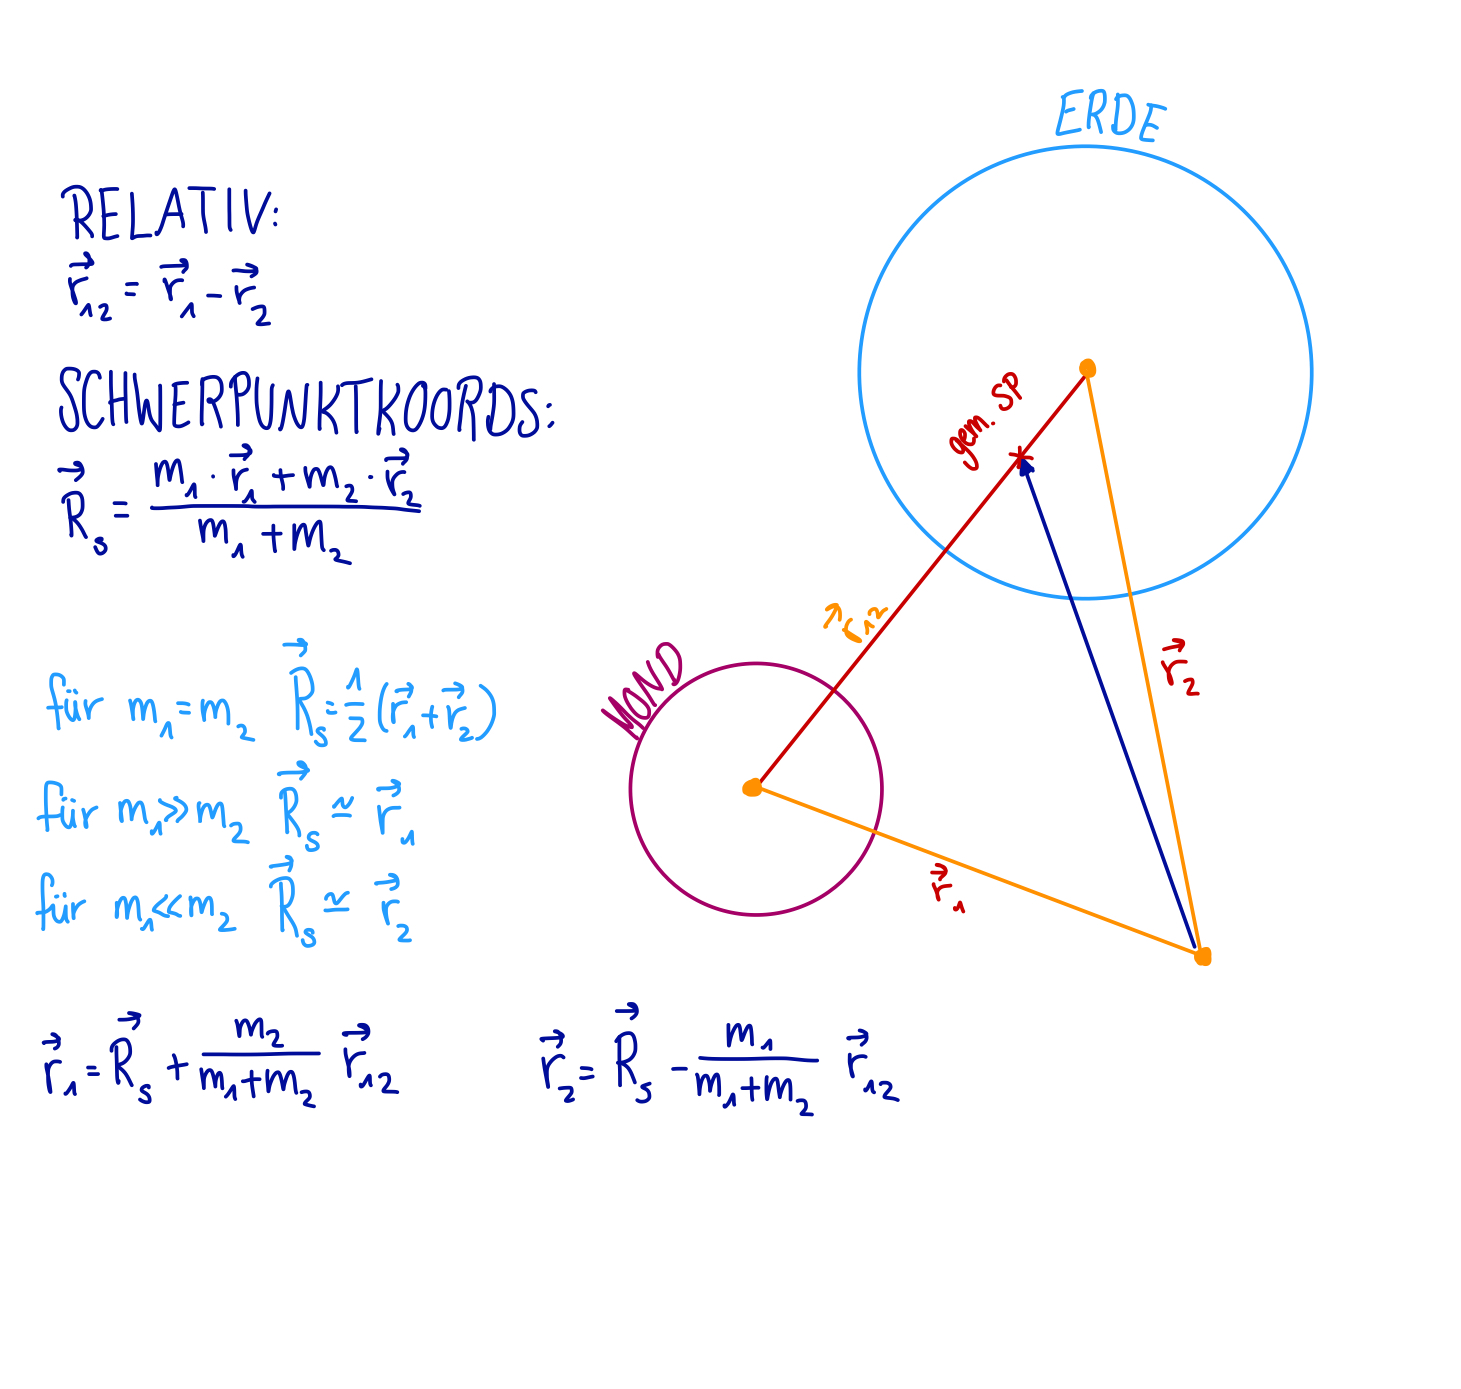
\includegraphics[scale=0.2]{IMG_7CD07FD55327-1.jpeg}
		\end{center}
		$\vec{v}_{12} = \dot{\vec{r}}_{}12 = \vec{v}_1 - \vec{v}_2 \qquad \vec{V}_S = \dot{\vec{R}}_S = \frac{m_1 \vec{v}_1+ m_2 \vec{v}_2 }{m_1 + m_2} $
		\[ M = m_1 + m_2 \]
		Für die reduzierte Masse: \[ \mu = \frac{m_1 \cdot m_2}{m_1 + m_2} [ \mu ] = kg \]
		für $ m_1 = m_2 \qquad \mu = \frac{1}{2} m_1 = \frac{1}{2} m_2 $\\
		für $ m_1 >> m_2 \qquad \mu \leq m_2 $
		\subsection{Gesamtimpuls}
			\[ \vec{p} = \vec{p} + \vec{p} = m_1 \vec{v}_1 + m_2 \vec{v}_2 \]
			Also 
			\[ \vec{p} = \mu \cdot \vec{V}_s \]
			$ \underbrace{m_1 \ddot{\vec{v}}_1 + m_2 \ddot{\vec{r}}_2}_{\dot{\vec{p}}} = \underbrace{\vec{F}_1 + \vec{F}_2}_\text{ Kraft außen}} $
		\[ \underbrace{\dot{\vec{p}} = \sum_{i, außen} \vec{F}_i }_{\text{Gesamtimpulsändung}}  \] 
		
\end{document}
